% Based on the official CVPR 2027 author kit, tag CVPR2027-v1.
\documentclass[10pt,twocolumn,letterpaper]{article}

\usepackage[review]{cvpr}
% Use \usepackage{cvpr} instead for the camera-ready version.
% !TeX root = main.tex
%% This file contains a number of tweaks that are typically applied to the main document.
%% They are not enabled by default, but can be enabled by uncommenting the relevant lines.


%%
%% Official support for 2-column teaser figure
%%
\usepackage{cuted} %< for strip environment

%%
%% For auto-referencing of figures (see fig/teaser.tex and \label{} therein) 
%%
\usepackage{currfile} %< for \currfilebase macro
\usepackage{microtype}
\usepackage{array}
\usepackage{xspace}
\newcommand{\method}{HereWeChoreography\xspace}

%%
%% caption and (global) spacing overrides
%%
\usepackage{caption} %< for "\captionof" commands (teaser)
% \setlength{\abovecaptionskip}{.5em} % space above caption
% \setlength{\belowcaptionskip}{1em} % space below caption

%%
%% Inline annotations; for predefined colors, refer to "dvipsnames" in the xcolor package:
%% https://tinyurl.com/overleaf-colors
%%
\newcommand{\red}[1]{{\color{red}#1}}
\newcommand{\todo}[1]{{\color{red}#1}}
\newcommand{\TODO}[1]{\textbf{\color{red}[TODO: #1]}}
%%
%% Disable for camera ready / submission by uncommenting these lines:
%%
% \renewcommand{\TODO}[1]{}
% \renewcommand{\todo}[1]{#1}

%%
%% Work harder in optimizing text layout. Typically shrinks text by 1/6 of page, enable
%% it at the very end of the writing process, when you are just above the page limit.
%%
% \usepackage{microtype}

%%
%% Fine-tune paragraph spacing.
%%
% \renewcommand{\paragraph}[1]{\vspace{.5em}\noindent\textbf{#1.}}

%%
%% Globally adjusts space between figure and caption.
%%
% \setlength{\abovecaptionskip}{.5em}

%%
%% Allows "the use of \paper to refer to the project name"
%% with automatic management of space at the end of the word.
%%
% \usepackage{xspace}
% \newcommand{\paper}{ProjectName\xspace}

%%
%% Commonly used math definitions.
%%
% \DeclareMathOperator*{\argmin}{arg\,min}
% \DeclareMathOperator*{\argmax}{arg\,max}

%%
%% Tighten underline.
%%
% \usepackage{soul}
% \setuldepth{foobar}

%%
%% Reconfigure paragraph (tweaks spacing)
%%

\usepackage[section]{placeins}
% Keep single-column supplementary figures close to their discussion.
\let\suppfigure\figure
\let\endsuppfigure\endfigure
\renewenvironment{figure*}[1][]{\suppfigure[!htbp]}{\endsuppfigure}
\let\supptable\table
\let\endsupptable\endtable
\renewenvironment{table}[1][]{\supptable[!htbp]}{\endsupptable}
\renewenvironment{table*}[1][]{\supptable[!htbp]}{\endsupptable}

\definecolor{cvprblue}{rgb}{0.21,0.49,0.74}
\usepackage{xr-hyper}
\usepackage[pagebackref,breaklinks,colorlinks,allcolors=cvprblue]{hyperref}
\externaldocument[][nocite]{ref-build/main}[main.pdf]

\def\confName{CVPR}
\def\confYear{2027}
\def\paperID{1134}

\DeclareRobustCommand{\herewechoreographyicon}{%
  \ensuremath{\vcenter{\hbox{%
    
\includegraphics[height=2.15em]{figures/title-icons/herewechoreography-title-icon.png}}}}%
  \hspace{0.5em}}
\title{\texorpdfstring{%
  \herewechoreographyicon
  \begin{tabular}[c]{@{}c@{}}
    HereWeChoreography\\
    Supplementary Material
  \end{tabular}%
}{HereWeChoreography Supplementary Material}}
\author{Anonymous CVPR submission}

\begin{document}
\onecolumn
\maketitle
\appendix
\renewcommand{\thefigure}{S\arabic{figure}}
\renewcommand{\thetable}{S\arabic{table}}
\renewcommand{\theequation}{S\arabic{equation}}
\renewcommand{\thepage}{S\arabic{page}}
% !TeX root = ../main.tex
\section{Annotation Components and Provenance}
\label{sec:annotation-details}
% !TeX root = ../main.tex
\begin{figure*}[t]
\centering
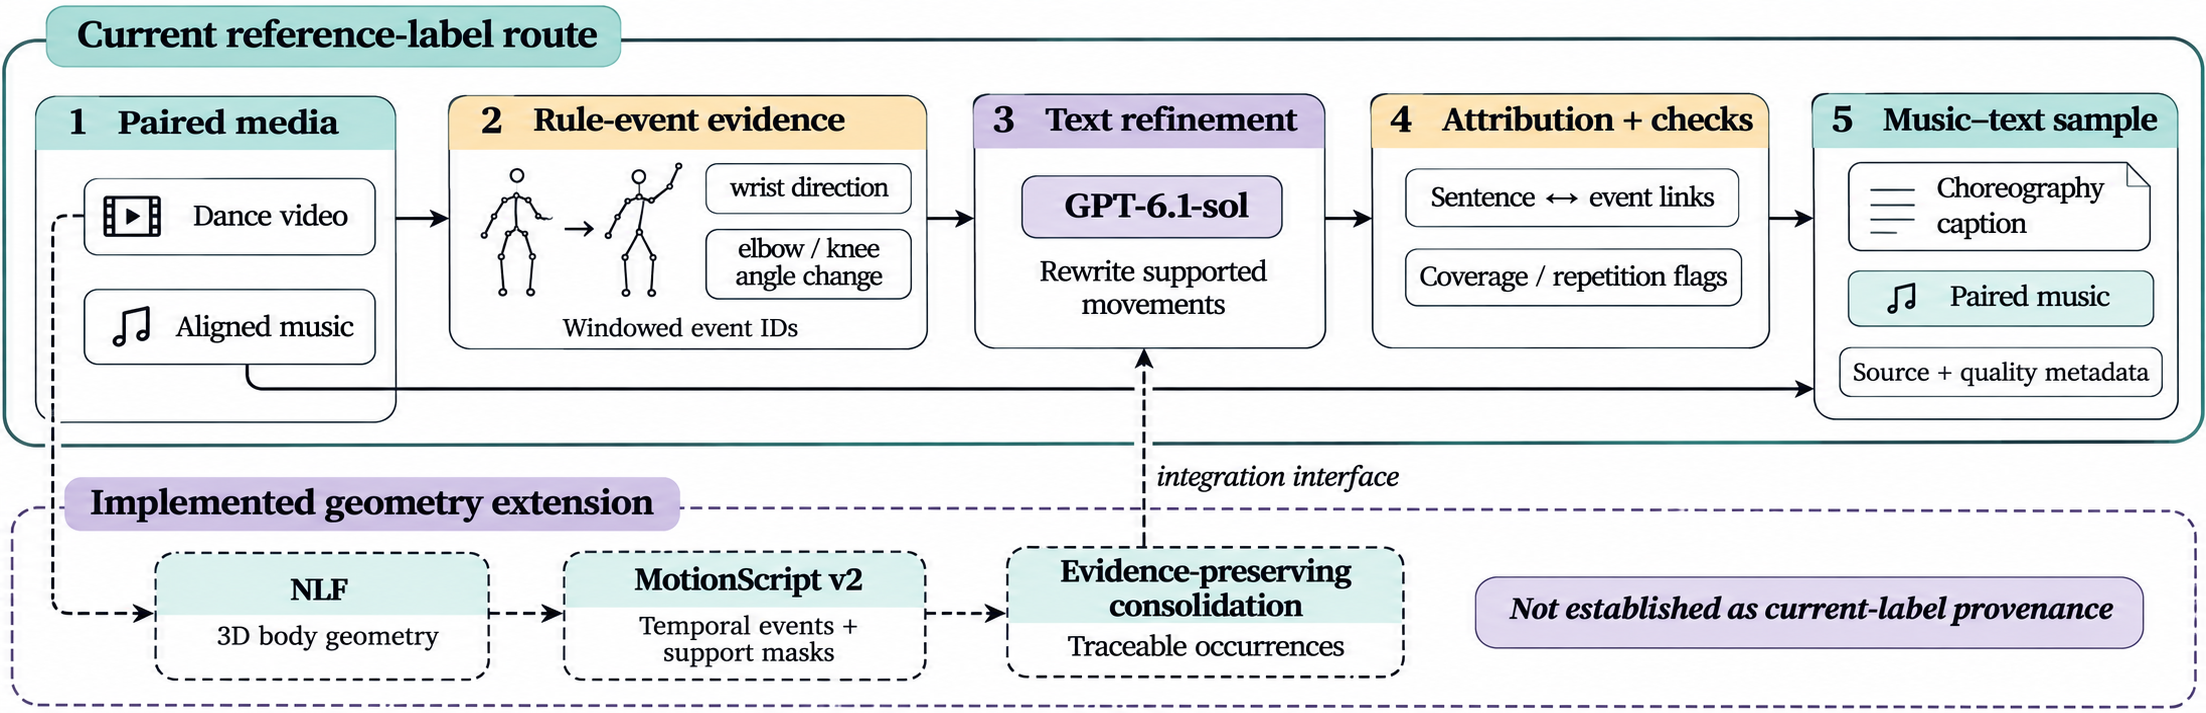
\includegraphics[width=\textwidth]{figures/dataset_construction_gpt_v2.png}
\caption{\textbf{Dataset construction with explicit provenance.}
The solid route produces current reference labels from windowed 2D
rule events through GPT-6.1-sol text refinement, attribution, and
automatic checks. Aligned music bypasses the refiner and is retained
in the final pair. The dashed NLF/MotionScript route is an implemented
extension whose integration into current labels is not established.}
\label{fig:dataset-construction}
\end{figure*}

The main-paper component-integration figure describes the implemented geometric
annotation route and the documented refinement interface. It is not
the established production history of the references used in the
captioning experiment. Those references come from the text-only
refinement of 2D rule-event logs described in Sec.~\ref{sec:data}.
In particular, neither a 20~FPS resampling operation nor additional
template joints introduces a new visual observation.

For descriptive analysis, original annotations and refined captions
were matched by identifier on 22,352 validation/test clips, retaining
all automatic quality flags. Original logs contain 47.21 event
statements per clip on average; refined descriptions contain 135.33
English body words and 5.12 producer-reported sentences. Wrist, elbow,
and knee events account for 60.3\%, 29.7\%, and 10.0\% of source-event
occurrences. These quantities have different units. They do not show
that the number of distinct observed actions increased or that
annotation accuracy improved. Source-style fields are unchanged;
unknown labels remain in the audited population and are reported in
the main text rather than excluded from the statistics.

\section{Composition and Targeted Revision}
\label{sec:revision-details}
% !TeX root = ../main.tex
\begin{figure*}[!htbp]
\centering
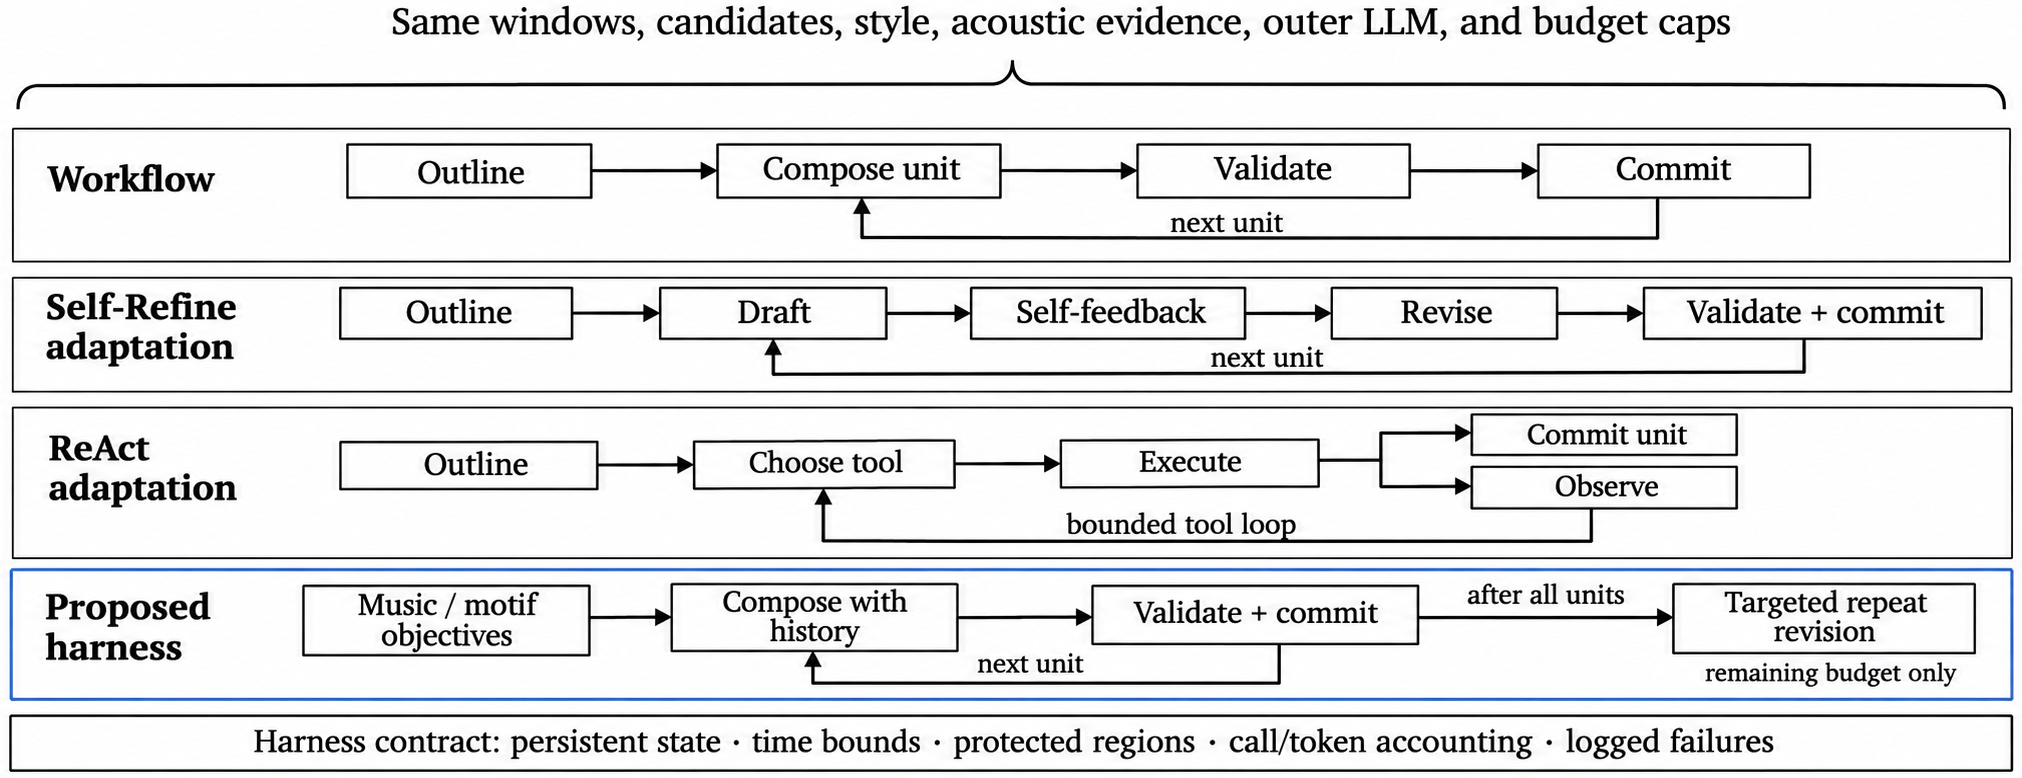
\includegraphics[width=\textwidth]{figures/agent_policy_comparison_gpt.png}
\caption{\textbf{Control-policy schematics for the shared-evidence comparison.}
Workflow uses direct composition, Self-Refine adds per-unit feedback and
revision, and ReAct selects tools through a bounded observation loop.
Commit observations advance ReAct to the next unit within that loop;
the displayed commit branch is a state update, not whole-song termination.
The proposed policy adds music/motif objectives and terminal targeted
revision with remaining budget. Common validation and failure handling
are abbreviated. These are implemented task adaptations, and this
figure reports no comparative quality result.}
\label{fig:agent-policy-comparison}
\end{figure*}

% !TeX root = ../main.tex
% Byte-preserved source and SHA: results/harness/controller_history.provenance.json.
% Historical 20261113 runs; not the current bar-aligned harness.
\begin{table}[t]
\centering
\caption{Earlier fixed-window controllers on 24 songs. Completion counts
legal final plans; mean calls includes all 24 attempts. These runs
predate the current bar-aligned harness.}
\label{tab:harness-controller-history}
\begingroup\footnotesize
\setlength{\tabcolsep}{4pt}
\renewcommand{\arraystretch}{1.08}
\begin{tabular*}{\columnwidth}{@{\extracolsep{\fill}}lrr@{}}
\toprule
Controller & Complete & Calls/song \\
\midrule
Workflow & 24/24 & 24.54 \\
Self-Refine & 24/24 & 71.63 \\
ReAct & 19/24 & 74.88 \\
Early choreography & 20/24 & 76.08 \\
\bottomrule
\end{tabular*}
\endgroup
\end{table}

% !TeX root = ../main.tex
% Provenance: results/harness/exploratory_ablation_repaired.provenance.json
% Use the repaired Section 17 results, not superseded ablation_v1.json.
\begin{table}[t]
\centering
\caption{Exploratory fixed-window ablations after timing repair ($n=4$). Qwen3-VL-8B rates text and acoustic summaries on four criteria (20 points); $\Delta$ is variant$-$W, averaged over orders, with 95\% song-bootstrap intervals. W lacks equal acoustic evidence: these are not isolated component effects or new bar-aligned results.}
\label{tab:harness-exploratory}
\begingroup\small
\setlength{\tabcolsep}{3pt}
\renewcommand{\arraystretch}{1.10}
\begin{tabular*}{\columnwidth}{@{\extracolsep{\fill}}lrr@{}}
\toprule
Variant & $\Delta$ & 95\% CI \\
\midrule
Q: motif quota & $+3.75$ & $[-1.63,\;7.25]$ \\
G: acoustic guidance & $+6.50$ & $[4.75,\;7.75]$ \\
S4: both & $+6.25$ & $[5.50,\;7.00]$ \\
\bottomrule
\end{tabular*}
\endgroup
\end{table}

Figure~\ref{fig:agent-policy-comparison} summarizes the four control
policies. Committed state and the remaining budget persist across unit
boundaries. Reading evidence or checking a draft does not advance the
song; a valid commit does. Only the proposed policy's predeclared
targeted revision stage may patch its selected completed spans.
A repeated movement can be an intentional
motif return. Candidate detection therefore identifies possible
redundancy for constrained revision, rather than determining artistic
quality. The current revision mechanism changes selected action text
while preserving its time bounds and protected regions. Boundary
reasoning remains text-based; it does not reconstruct an unobserved
physical state.

\section{Diagnostic Metrics and Style Protocols}
\label{sec:experimental-details}
% !TeX root = ../main.tex
% Supporting diagnostics; requires booktabs.
\begin{table*}[!htbp]
\centering
\caption{Full-2000 lexicon diagnostics and evaluation coverage. These are supporting statistics, not additional independent choreography-quality experiments.}
\label{tab:e2-full2000-diagnostics}
\begingroup\small
\setlength{\tabcolsep}{3pt}\renewcommand{\arraystretch}{1.12}
\begin{tabular*}{\textwidth}{@{\extracolsep{\fill}}lrrrrrr@{}}
\toprule
\multicolumn{7}{l}{\textbf{A. Micro-averaged lexicon agreement (all values $\times 100$)}}\\
\midrule
Method & KW-P & KW-R & KW-F1 & BP-P & BP-R & BP-F1 \\
\midrule
Qwen3-Omni-Instruct & 35.09 & 24.67 & 28.97 & 50.39 & 74.69 & 60.18 \\
MOSS-Audio & 17.58 & 5.83 & 8.76 & 54.71 & 13.23 & 21.31 \\
MOSS-Music & 15.42 & 9.80 & 11.99 & 49.73 & 53.81 & 51.69 \\
Music-Flamingo & 32.03 & 14.19 & 19.67 & 29.17 & 14.60 & 19.46 \\
Audio-Flamingo3 & 20.00 & 6.02 & 9.25 & 81.67 & 6.52 & 12.08 \\
Qwen2.5-Omni & 7.93 & 2.84 & 4.18 & 72.54 & 20.60 & 32.09 \\
\textbf{SFT v3 (ours)} & \textbf{76.23} & \textbf{85.90} & \textbf{80.78} & \textbf{91.66} & \textbf{96.72} & \textbf{94.12} \\
\bottomrule\end{tabular*}\par\vspace{9pt}
\begin{tabular*}{\textwidth}{@{\extracolsep{\fill}}lrrr@{}}
\toprule
\multicolumn{4}{l}{\textbf{B. BERTScore coverage and original available-case means}}\\
\midrule
Method & Valid / 2,000 & Coverage (\%) & Available-case F1 $\times100$ \\
\midrule
Qwen3-Omni-Instruct & 1,999 & 99.95 & 78.49 \\
MOSS-Audio & 1,999 & 99.95 & 82.63 \\
MOSS-Music & 1,998 & 99.90 & 82.13 \\
Music-Flamingo & 1,865 & 93.25 & 82.29 \\
Audio-Flamingo3 & 2,000 & 100.00 & 82.20 \\
Qwen2.5-Omni & 2,000 & 100.00 & 82.85 \\
SFT v3 (ours) & 2,000 & 100.00 & 89.71 \\
\bottomrule\end{tabular*}\par\vspace{9pt}
\begin{tabular*}{\textwidth}{@{\extracolsep{\fill}}lrrrr@{}}
\toprule
\multicolumn{5}{l}{\textbf{C. Surface diagnostics (no quality ranking)}}\\
\midrule
Method & BV $\times100$ & TC present / 2,000 & Duplicate excess & Length ratio \\
\midrule
Qwen3-Omni-Instruct & 13.03 & 1,721 & 12 & 1.388 \\
MOSS-Audio & 2.01 & 1,996 & 801 & 0.544 \\
MOSS-Music & 10.75 & 1,617 & 16 & 0.995 \\
Music-Flamingo & 7.93 & 1,848 & 626 & 0.750 \\
Audio-Flamingo3 & 0.77 & 1,985 & 1,357 & 0.285 \\
Qwen2.5-Omni & 5.45 & 1,998 & 1,398 & 0.281 \\
SFT v3 (ours) & 43.23 & 2,000 & 0 & 1.063 \\
\bottomrule\end{tabular*}
\par\vspace{5pt}
\begin{minipage}{\textwidth}\footnotesize
\textbf{Reading the diagnostics.} BERT coverage is a measurement-availability statistic, not a quality score. Original means in B use different valid sets and should not be subtracted as paired effects. BV is body-part/verb co-occurrence; TC counts texts containing a temporal connective, not correct temporal relations. Duplicate excess is $N-U$, where $U$ is the number of distinct exact text strings; it is not the count of every sample belonging to a duplicate cluster. A zero does not establish semantic novelty. TC counts and duplicate excess are exact re-expressions of the archived rates, not newly computed semantic metrics. Length ratio is the mean generated/reference character ratio; a value near one is not a quality target. All seven methods returned 2,000 texts. KW and BP inventories are coarse and partly overlapping.
\end{minipage}
\endgroup\end{table*}

The diagnostics retain each method's evaluation coverage and
available-case BERTScore in addition to the common-case main comparison.
An exact duplicate count measures identical returned strings, not
semantic movement diversity. Table~\ref{tab:style-prior-822} reports
only the 822-clip style population, retaining all seven zero-shot models
and all three supervised objectives on the same clips.

\paragraph{Automatic-rating configuration and coverage.}
For Table~\ref{tab:refinement-d123}, \emph{Ours} denotes the supplied
task-specific captioner predictions. Released processing-stage metadata
disagree with the author-reported generation configuration, so the
output-stage lineage remains unresolved. These ratings alone are not
an isolated ablation of supervised fine-tuning.
The Ours release comes from public commit \texttt{dc6dfd9}; the baseline
release comes from \texttt{92d6dcf}. All eight generation inventories
contain the same 2,000 case IDs. All released outputs are retained in
the audit, alongside a separate record of the configuration clarification.
Scores marked invalid or null
are omitted per dimension, never replaced with zero. The public export
contains numeric scores and status fields, without response bodies,
evidence quotations, assessor identity, or acoustic-input metadata.
The main comparison uses the recorded r4 scoring family, the only
published version available for every method. Baselines provide r4
judgments on the same 1,900 holdout IDs; Ours is restricted to those
IDs before aggregation. Each dimension then uses the common valid
intersection across all eight methods: 1,888 for Q1, 1,833 for Q2,
and 1,858 for Q3. The shared valid-case means, per-method available-case
means, missing statuses, and ID hashes are preserved in the audit.
The older baseline v1.2 run is not mixed into the comparison.

For sensitivity on the complete Ours release, r4 yields 4.97/3.33/4.80
and v2.1 yields 4.92/4.50/4.91. v2.1 was defined after earlier tests;
it is excluded from the main comparison because compatible baseline
judgments were not released. No per-dimension maximum across versions
is selected. The baseline manifest identifies the r4 version by name,
but omits the rubric content hash, so exact prompt-hash parity cannot
be independently established from the export.
Published record IDs D1--D3 are displayed as Q1--Q3 without changing
their numerical values. The revised M3 affect criterion replaces the
earlier local-development design; no legacy development scores are reused.
These records cannot establish calibration to our nine-dimensional
anchors. Differences between protocols are not model improvements, and
reference agreement has not been recomputed on the supplied rating outputs.
Full-release Ours Q1/Q2/Q3 valid counts are 1,999/1,990/1,999 for r4
and 2,000/1,966/1,999 for v2.1; these available-case values are not
substituted for the common-case main table. The earlier two-axis
baseline assessment is likewise not relabeled as these three dimensions.

\paragraph{Caption decoding and metric configuration.}
Reference agreement uses 2,000 clips; BERTScore uses the common
1,861 valid cases for every method, while the other main-table reference
metrics use all clips.
The reported SFT checkpoint uses temperature 0.7, top-$p$ 0.9,
top-$k$ 20, one beam, repetition penalty 1.05, no-repeat 4-grams,
at most 1,024 generated tokens, and an explicit chat EOS. A per-case
sampling seed is derived from its identifier. The baseline stopping
metadata are incomplete; a returned text does not by itself prove
that generation was untruncated. BERTScore is computed without silent
truncation on the common valid intersection; the available-case
statistics use different case sets and cannot be subtracted as paired
effects.

\paragraph{Style pseudo-labels and supervision.}
The 822-clip style population uses video-VLM pseudo-labels, rather than
human judgments of music--dance suitability. Rankings use 22 labels;
Macro-F1 and balanced accuracy average over the 13 classes observed in
this population. Eight classes have 100 examples each; the other five
have 1, 1, 1, 3, and 16 examples. Class-balanced scores are therefore
descriptive and sensitive to very scarce classes.

The frozen MuQ encoder supplies features to three supervised heads:
cross-entropy, weighted cross-entropy, and focal loss. Positive training
examples cover only 15 of 22 outputs. Focal was selected by validation
Macro-F1, then balanced accuracy and unweighted NLL, before inspecting
this preview; scalar-temperature calibration uses separate calibration
data. The paired focal-minus-cross-entropy 95\% intervals are
$[-2.43,3.53]$ points for Top-1 and $[-2.68,1.70]$ for Top-3.
Seven unsupported outputs prevent a complete 22-class training claim.
Neither classification agreement nor these objective comparisons establish
that conditioning a harness on the predicted style improves choreography.

\section{Implementation and Validation Details}
\label{sec:remaining-tests}
% !TeX root = ../main.tex
\paragraph{Observation and planning contracts.}
The candidate cache retains the source audio identity, exact observation
intervals, model configuration, and generation provenance. Proposals
are compositional evidence rather than ground-truth action sequences
or instructions that must be copied verbatim. Extending the planning
horizon does not require the captioner to describe an entire song in
one response. The outline and committed history supply long-range
context beyond local proposals.

\paragraph{Reproducible controller defaults.}
The candidate collector defaults to two proposals per observation window.
The controlled experiment runner uses up to five repetition groups;
older runs may use the underlying controller's three-group default and
must retain their recorded configuration. Grouping compares normalized
token sets against a representative action at Jaccard similarity
$\geq0.80$. The first occurrence stays fixed. Replacement text is accepted
only when its overlap with the representative lies between 0.20 and
0.80 and the patch passes structural validation. This vocabulary guard
does not verify semantic correctness. Each selected group receives at
most one request within the remaining outer budget. Time, track, motif,
evidence, and other protected event fields remain unchanged.

\paragraph{Clock and cost accounting.}
Observation and event boundaries use integer samples on the canonical
audio clock. Exported review cases divide these boundaries by the source
sample rate to obtain global seconds, retaining the original offset for
audio crops. Shared audio preparation and candidate collection are
accounted for separately from outer composition. The $1+4U$ outer-call
limit is an upper bound, not a fixed inference cost. Client-visible
dispatches and their usage are recorded; any hidden service retry
requires separate tracing before physical-request totals can be claimed.
The cached proposal and evidence configuration is fixed for the new
controlled comparison, while historical results retain their original
conditions.

\paragraph{Variable-duration deployment.}
The bar partition supplies both observation intervals and planning units.
Leading and trailing incomplete bars remain explicit fragments; a short
fragment may merge with a neighbor in the same public section.
Insufficient downbeat evidence or an unsupported duration requires
review rather than silent fallback to fixed windows. Audio is neither
stretched nor implicitly truncated to match the target duration.
Variable-duration captioner consumption requires server preflight:
successful partitioning and waveform loading do not establish that the
model's processor consumes the entire waveform or preserves caption
quality. The current variable-duration collection path uses a native
model resident in one process; the legacy fixed-duration service
contract cannot substitute for this path. These deployment checks have
not yet been reported as completed model experiments.

\paragraph{Global condition and evidence.}
The style predictor may retain its native short observation windows
independently of the choreography partition. Duration-weighted pooling
gives overlapping observations shared ownership of their common span.
The resulting label is a creative prior rather than a unique correct
dance genre. The composer consumes cached captions and acoustic
summaries; it has no additional raw-audio listening tool inside the
current composition loop. An unavailable or uncertain signal must remain
explicit rather than be replaced with an invented musical label.

\paragraph{Scoped editing interface.}
For editing, the user supplies an instruction and target regions or
event identifiers. A version-bound patch declares editable targets,
protected fields, and any explicitly permitted boundary-repair events.
Changes outside this scope are rejected; accepted operations are
applied transactionally and the resulting score is validated. This
protects unrelated choreography, while semantic fulfillment of the
request requires separate evaluation. The interface does not establish
the physical feasibility of an unrendered dance, and a validated
user-editing experiment is not included in the current results.

The controlled comparison preserves failed and partial runs in its
registered inventory. It requires no additional model training.

Two implemented revision controls reuse the actual saved drafts:
the proposed harness before its terminal revision, and the Workflow
draft passed through the same revision mechanism with its remaining
budget. They isolate structured composition from simply adding more
rewriting. Further ablations can compare true bar-aligned versus fixed
windows, remove the global style condition, or permute acoustic evidence
from an immutable source copy. They require independent runs and are
not assigned numerical outcomes in this draft.

The latest implementation has static syntax and consistency checks;
its real variable-duration model input and audio-judge coverage still
require server validation. The 2,000-clip reference panel also needs a
final training/checkpoint provenance audit before it can support a
strictly unseen-data generalization claim. The evaluation report names
the v3 base model and joint-aware clause weighting. The released
implementation and checkpoint report specify a lower-limb vocabulary
and a coefficient of 1.5. The original run configuration and source
hashes are still needed to verify the exact training scope, optimizer
schedule, batch size, and record filter. A controlled comparison
against trained-model-disabled decoding would further isolate the
effect of adaptation. A listener study, rubric sensitivity controls,
and human--model agreement are needed before the new rubric can be
presented as a validated automatic quality metric.

\paragraph{Joint-aware clause reweighting.}
The released configuration targets clauses naming leg, knee, thigh,
shin, calf, hamstring, or quad. Clause boundaries follow commas,
semicolons, and sentence stops. With tokenizer offsets, all overlapping
clause tokens receive the weight; an offset-mapping fallback marks
matched part tokens only. Weighted cross-entropy is normalized by the
unweighted number of valid assistant tokens, not by the sum of weights.
The development report records lower-limb mention coverage of 0.993
in references versus 0.787 in baseline outputs, motivating the selected
region. These are lexical diagnostics, not joint-motion accuracy.
A random-clause control has not been run, so version differences cannot
be attributed solely to the semantics of the selected joints.

\paragraph{Reference-metric calculation.}
For a predicted category set $P_i$ and reference set $R_i$, the pooled
counts are $\mathrm{TP}=\sum_i|P_i\cap R_i|$,
$\mathrm{FP}=\sum_i|P_i\setminus R_i|$, and
$\mathrm{FN}=\sum_i|R_i\setminus P_i|$. The reported lexicon score is
\begin{equation}
 F_{1,\mathrm{micro}}=
 \frac{2\mathrm{TP}}{2\mathrm{TP}+\mathrm{FP}+\mathrm{FN}}.
\end{equation}
The same definition is applied separately to the motion-keyword and
body-part inventories; it is not a score for binding the two. Token-F1
uses token multiplicity rather than binary category membership.
ROUGE-L uses longest-common-subsequence overlap; BERTScore uses
contextual token matching. Corpus BLEU-4 is displayed after multiplication
by 100, so a table value above one is consistent with its scale.
There is no additional undocumented normalized-BERT composite in the
main comparison. BERTScore's raw F1 and its valid-case coverage are
reported explicitly.

\paragraph{Plan diagnostics.}
For a song of duration $T$ and written action intervals $I_k$, temporal
coverage is $|\bigcup_k(I_k\cap[0,T])|/T$. This measures how much time
has a scheduled description, not whether the dancer follows the beat.
Exact duplicate excess is $N-U$, where $U$ is the number of unique
returned strings. Near-text similarity identifies potential repeated
wording; neither measure can distinguish a desirable recurring motif
from unproductive copying without context. Confirmed boundary conflicts
should count only explicit incompatible states and report the number
of boundaries for which sufficient evidence exists.

\paragraph{Historical mechanism diagnostics.}
The earlier repetition-repair experiment counts normalized exact
strings within each plan: $d_s=1-U_s/N_s$, where $N_s$ is its number
of action entries and $U_s$ its number of unique normalized strings.
Normalization lowercases text, replaces non-alphanumeric characters
with spaces, and collapses whitespace. The main-text 73.14\% and 36.82\%
are means over five paired song records, not a pooled event-level rate;
the sixth registered record has no valid pair. This early variant
rewrites at most three groups. It differs from both the cosine-based
near-duplicate diagnostic and the latest five-group Jaccard-based
revision mechanism. Their rates cannot be combined.

The repaired four-song ablation supersedes the earlier timing-unit
results. Its songs participated in development, and the archived
summary does not fully establish label blinding and action-text
presentation limits. We retain its uncertainty intervals as exploratory
evidence. In a separate six-song presentation audit, extending visible
action text from 160 to 400 characters removes the apparent advantage
of more restrictive rewriting over its predecessor: $0.00\;[-2.00,2.00]$.
This is a sensitivity result, not confirmation of equivalent quality.
An identical-plan control has seven parsed pairs of eight registered;
its two-order mean difference is zero, but six of 56 dimension-level
comparisons still favor a presentation position. Order averaging
therefore does not establish an unbiased judge.

\paragraph{Quality summaries and uncertainty.}
The proposed rubric keeps each dimension separate. For local evaluation,
the three common regions are first averaged within each song using the
scored regions for that dimension. A song-level mean then gives each
song equal weight, with valid-region and valid-song counts reported.
Unknown judgments are not replaced by zeros.
Comparisons use paired song differences; source-group bootstrap draws
resample songs together with all of their regions. The planned primary
comparisons are the proposed method against each of the three baseline
policies on G1--G3; multiplicity control and the primary judge must be
frozen before examining results. These aggregation rules specify the
next experiment and do not imply that new rubric scores already exist.

\section{Limitations and Responsible Use}
The current labels inherit the observational limits of their source
events and do not supply unique correct dances for music. Projected
directions do not always identify anatomical laterality. Missing or
occluded body regions can produce uncertain geometry, and richer
wording must not be interpreted as new visual evidence. The global
style classifier is a supervised creative prior evaluated against
video-derived pseudo-labels; it is neither a universal music-genre
classifier nor an authority on culturally appropriate choreography.

The outer composer uses summarized evidence, rather than direct raw
audio in its tool loop. Its checks verify a written schedule and
explicit textual constraints, not balance, joint limits, contact, or
injury risk. Precise editing is supported by scoped permissions, but a
validated user-editing experiment is not included here. Dataset release
must respect the licenses and permissions of the underlying music and
videos; these rights cannot be inferred from the availability of
derived captions.

\section{Detailed Rubric and Calibration Guide}
\label{sec:rubric-guide}
% !TeX root = ../main.tex
% Condensed from tables/rubric_anchors_detailed.tex; no additional scoring standard.
\begin{table*}[t]
\centering
\caption{Core anchors of the proposed rubric. Scores 1 and 5 require dimension-specific evidence; intermediate anchors and exceptions appear in Table~\ref{tab:rubric-detailed-anchors}. Calibration remains pending.}
\label{tab:rubric-core-anchors}
\begingroup\small
\setlength{\tabcolsep}{4pt}
\renewcommand{\arraystretch}{1.10}
\begin{tabular}{@{}>{\raggedright\arraybackslash}p{0.15\textwidth}>{\raggedright\arraybackslash}p{0.405\textwidth}>{\raggedright\arraybackslash}p{0.405\textwidth}@{}}
\toprule
Dimension & 1: core failure & 5: supported fulfillment \\
\midrule
D1: Specificity & Mood/style or generic dancing leaves the main movement unidentifiable. & Main movements and necessary attributes are explicit, without inventing the action. \\
D2: Body/space & Explicit body, spatial, reference-frame, or concurrent-action relations conflict. & Necessary body/spatial relations are clear and compatible, including concurrent actions. \\
D3: Local timing & Order/duration conflicts; clearly serial actions exceed available time. & Order, concurrency, sustained actions, and transitions fit the interval coherently. \\
D4: Rhythm & Claimed rhythm contradicts audible pulse/pauses, or movement rhythm is unspecified. & Repetition, pauses, speed, or movement density correspond to audible rhythm. \\
D5: Expression & Claimed force/articulation conflicts with, or depends on absent, audible features. & Force, articulation, or sustained motion responds to audible expression or grounded contrast. \\
D6: Development & Invents a key musical change, or an applicable change lacks a movement response. & Movement maintenance, emphasis, or change relates to independently identified musical development. \\
\midrule
L1: Continuity & Important boundaries impose incompatible explicit states without a resolving transition. & Important boundaries connect coherently, without decisive explicit state conflicts. \\
L2: Global structure & Unorganized concatenation or explicit conflict with audible whole-song structure. & Section functions and overall progression coherently reflect musical development. \\
L3: Motifs/variation & Unorganized repetition or unrelated changes prevent recognizable thematic development. & Recognizable motifs recur, extend, or vary at musically justified positions. \\
\bottomrule
\end{tabular}
\endgroup
\end{table*}

% !TeX root = ../main.tex
% Dimension definitions: notes/54_benchmark_rubric_ablations_and_case_studies_20261114_zh.md.
% Executable identifiers/common scale: experiments/structured_dev_20261114/judge_rubric_v2.py.
% This table is a recommended calibration guide, not a completed validation study.
\begin{table}[!htbp]
\centering
\caption{Detailed anchors for the proposed evaluation protocol. The executor implements the nine dimension identifiers and common 1--5 scale. The dimension-specific anchors below are a \textbf{recommended calibration guide}, not validated scoring thresholds or completed calibration results. Judge only the supplied music and timed action text.}
\label{tab:rubric-detailed-anchors}
\begingroup\small
\setlength{\tabcolsep}{4pt}
\renewcommand{\arraystretch}{1.11}
\begin{tabular}{@{}>{\raggedright\arraybackslash}p{0.13\textwidth}p{0.27\textwidth}p{0.27\textwidth}p{0.27\textwidth}@{}}
\toprule
Dimension & 1: severe defect & 3: usable but important omission & 5: supported fulfillment \\
\midrule
D1: Movement specificity & Core movement cannot be identified; text mainly states mood, style, or generic dancing. & Main movement is identifiable, but an attribute essential to interpreting it is missing. & Core movements and necessary attributes are explicit, without requiring the reader to invent the main action. \\
\addlinespace
D2: Body/spatial consistency & Explicit body-part, laterality, reference-frame, or simultaneous-action relations conflict. & Most relations are understandable, but an important direction, referent, or coordination relation is ambiguous. & Necessary body/spatial relations are clear and mutually consistent; simultaneous actions are compatible as written. \\
\addlinespace
D3: Local temporal organization & Explicit order, concurrency, or duration requirements conflict, or clearly serial actions exceed the available time. & The local sequence is intelligible, but a consequential duration, transition, or temporal dependency is underspecified. & Ordering, concurrency, sustained actions, and transitions fit the stated interval without an explicit timing conflict. \\
\addlinespace
D4: Rhythmic response & Asserted rhythmic correspondence contradicts audible pulse/pauses, or no assessable movement rhythm is specified. & Movement rhythm broadly fits, but its connection to a specific audible pattern is weak or incomplete. & A concrete relationship links movement repetition, pauses, speed, or density to audible rhythm; justified half-time remains valid. \\
\addlinespace
D5: Expressive response & Claimed force or articulation correspondence relies on an absent musical feature or a clear unsupported conflict. & The broad expression is compatible, but movement force, release, articulation, or its musical rationale remains generic. & Specific force, articulation, or sustained movement responds to audible expression, including a clearly grounded intentional contrast. \\
\addlinespace
D6: Local development response & Invents a key musical change, or an applicable change has no interpretable movement response. & Some movement development is described, but its relation to the independently identified musical change is incomplete. & Maintaining, emphasizing, or changing movement has a clear relationship to the independently identified audible development. \\
\midrule
L1: Cross-window continuity & Important neighboring windows impose explicitly incompatible states with no resolving transition. & Most boundaries connect, but an important transition remains ambiguous or insufficiently explained. & Important boundaries admit coherent transitions; no decisive explicit state conflict remains across neighboring windows. \\
\addlinespace
L2: Global development & The score is predominantly unorganized concatenation or clearly conflicts with the audible whole-song structure. & A global arrangement exists, but section roles, contrast, or progression are weakly connected. & Section functions and overall progression form a coherent plan grounded in the music's actual development. \\
\addlinespace
L3: Motif recurrence/variation & Templates repeat without musical organization, or unrelated changes prevent recognizable thematic development. & Recognizable motifs and variation occur, but some returns or changes lack a clear organizing rationale. & Recognizable motifs recur, extend, or vary at musically justified positions; repeated material has a coherent purpose. \\
\bottomrule
\end{tabular}
\par\vspace{5pt}
\begin{minipage}{\textwidth}\footnotesize
\textbf{Intermediate scores.} Score 2 retains some useful content but has a critical defect; score 4 meets core requirements with only minor deficiencies. Scores 4--5 require a concrete correspondence, not generic claims of suitability. One defect affects multiple dimensions only when its consequences independently warrant each deduction.
\par\smallskip
\textbf{Evidence.} Every numeric score requires an exact quotation, cited event identifiers, and a reason. D4--D6 and L2--L3 additionally require an audible observation and an interval on the global song clock. Quote matching and timestamp validation check the response contract, not semantic correctness or actual model listening.
\par\smallskip
\textbf{Unknown and applicability.} Insufficient observable evidence gives \emph{unknown}, with no numeric score; assessable vagueness or poor content instead receives a low score. Only D6 permits \emph{not applicable}, when its audio-only applicability decision was frozen as false before candidates were inspected. Unresolved D6 applicability gives unknown for every method. Missing audio, service errors, and parsing failures retain distinct failure records and count toward coverage reporting.
\par\smallskip
\textbf{Creative latitude.} Do not require extra joints, longer descriptions, faster movement, or a change at every musical event. Sustained movement, silence, half-time, contrast, and motivated repetition are legitimate. An unspecified support foot alone is not an explicit contradiction. D3 concerns the written local schedule; L1 concerns boundaries between windows. Neither measures biomechanics of an executed dance.
\end{minipage}
\endgroup
\end{table}

The anchors distinguish requirements for local movement, music response,
and whole-song organization. Before collecting formal scores, calibration
should test claim-specific musical contrasts, compatible cross-song reuse,
explicit body/timing conflicts, unproductive copying, and legitimate motif
returns on frozen examples. A choreography need not identify a unique song.
Neither a visually clear rubric nor successful response validation
establishes agreement with independent listeners.

\paragraph{AI assistance.}
Language models assisted with drafting and revising manuscript text,
literature organization, code, and experiment planning. GPT Image
produced early conceptual illustrations; the current diagrams were rebuilt
as editable vector objects, and statistical panels reproduce frozen
audit values. GPT-6.1-sol participates in annotation refinement.
Numerical results come from saved experiment artifacts. The authors
retain responsibility for the manuscript, citations, figures, code,
data provenance, results, and final submission declarations.

\end{document}
